\chapter{Planning of tracker calibration}
\textit{Reconstructing cosmic tracks and understanding resolutions require calibrating the tracker station \ref{trackersec}. 
The main goal of this calibration is to determine signal propagation and channel-to-channel delays for each straw. 
To do this, an unbiased reconstruction of the track longitudinal position in a straw is needed.
In this chapter, I will discuss the planning of the calibration with cosmic muons. My task involved reconstructing 
the cosmic trajectories in a station oriented vertically. This orientation introduces biases and systematics that 
need to be understood before the data taking.  }
\section{Calibration of the station with cosmic muons}
Cosmic muons serve as a crucial calibration source for the Mu2e detector system, particularly for the tracker station. 
They possess unique characteristics that make calibration with cosmic rays complementary to other techniques:
\begin{itemize}
    \item they can be acquired during standard run operations, under the same experimental conditions as the physics data sample;
    \item their flux ($\sim 1 \ \text{cm}^{-2} \text{min}^{-1}$ for horizontal detectors with a mean
    energy of $\sim$4 GeV, Ref. \cite{muonflux}) is sufficiently high to gather a substantial amount of calibration data in a short period, 
    enabling continuous monitoring of the detector response;
    \item as minimum ionizing particles (MIPs), their energy loss is almost independent of their initial energy;
    \item being relativistic particles with negligible energy loss, their speed is almost always equal to the speed of 
    light $c$. The time they take to traverse the station can be used to align the time offsets of all the channels without any external time reference.
\end{itemize}
\subsection{Distribution of the cosmic muons energy and angle}
The muon flux at sea level is usually described by the standard Gaisser's formula, Ref. \cite{guan2015parametrization}:
\begin{equation}
    \frac{d I}{d E_\mu d \Omega d t d S}=\frac{0.14}{\mathrm{~cm}^2 \mathrm{~s} \ \mathrm{sr}}\left(\frac{E_\mu}{\mathrm{GeV}}\right)^{-2.7} \quad\left[\frac{1}{1+\frac{1.1 E_\mu \cos \theta}{115 \mathrm{GeV}}}+\frac{0.054}{1+\frac{1.1 E_\mu \cos \theta}{850 \mathrm{GeV}}}\right]
    \end{equation}
where $E_\mu$ is the muon energy and $\theta$ is the polar angle of the muon. 
The two terms in brackets correspond to the contribution of the charged pions and kaons, while 
the small contribution from charm and heavier flavors is neglected. 
This simplified formula doesn't take into account muon decays and the curvature of the Earth, 
thus it is only valid for zenith angles $\theta < 70^\circ$ and for energies $E > \frac{100}{\cos \theta}$ GeV.
A modified version of the standard Gaisser formula, called Gaisser Tang model, is used to account for low energy and large zenith angle effects, Ref. \cite{guan2015parametrization}:
\begin{equation}\label{cosmicmuonflux}
    \frac{d I}{d E_\mu d \Omega d t d S}=\frac{0.14 E_\mu}{\mathrm{cm}^2 \mathrm{~s} \ \mathrm{sr} \ \mathrm{GeV}}\left(1+\frac{3.64 \mathrm{GeV}}{E_\mu\left(\cos \theta^*\right)^{1.29}}\right)^{-2.7}\left[\frac{1}{1+\frac{1.1 E_\mu \cos \theta^*}{115 \mathrm{GeV}}}+\frac{0.054}{1+\frac{1.1 E_\mu \cos \theta^*}{850 \mathrm{GeV}}}\right]
\end{equation}
where second term in the bracket is the same as in the standard formula, except that the zenith angle 
$\theta$ is substituted by the angle $\theta^*$. The relation between cos$\theta$
and cos$\theta^*$ is given by:
\begin{equation}
    \cos \theta^*=\sqrt{\frac{(\cos \theta)^2+P_1^2+P_2(\cos \theta)^{P_3}+P_4(\cos \theta)^{P_5}}{1+P_1^2+P_2+P_4}}
    \end{equation}
The parameters $P_1$ = 0.102573, $P_2$ = -0.068287, $P_3$ = 0.958633, $P_4$ = 0.0407253, and $P_5$ = 0.817285 were calculated using 
a dedicated simulation of muon production in the atmosphere. A representation of the angles is shown in Figure \ref{fig:anglesinmuon}.
Another factor is included in Equation \ref{cosmicmuonflux} to account for the possibility of muon decays, which are more 
significant at low energies. The numerical constants are derived by fitting experimental data from various cosmic muon studies.
\begin{figure}[!h]
    \centering
    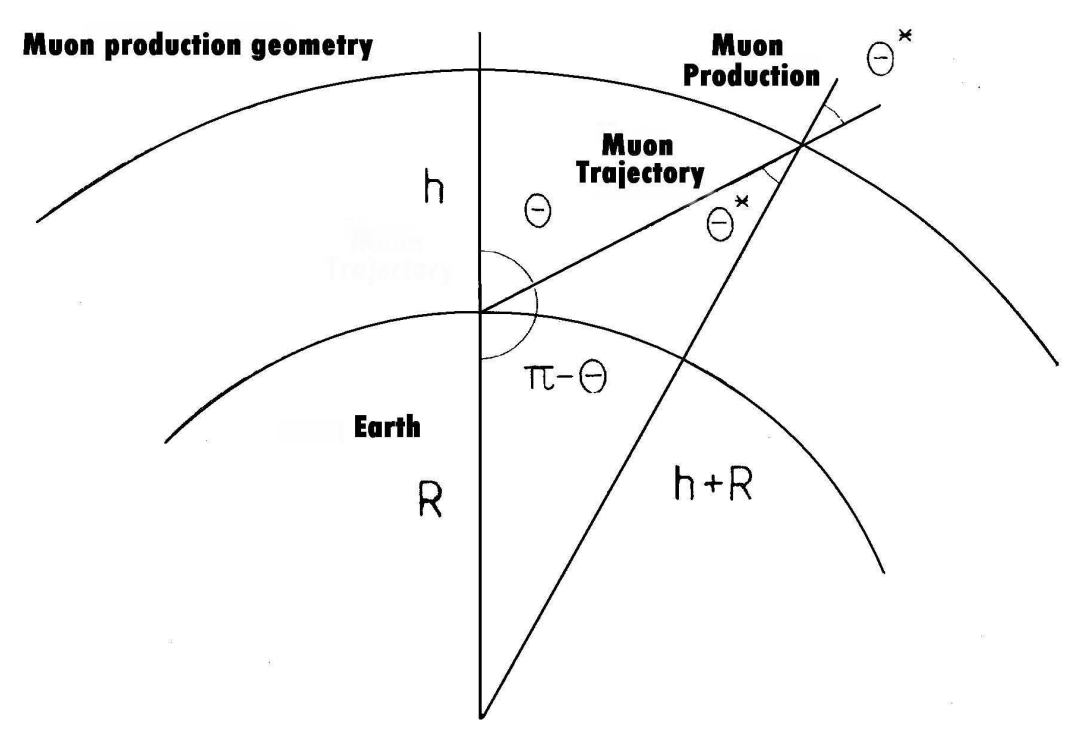
\includegraphics[width =0.6\textwidth]{figures/png/Screenshot_20240526_140716.png}
    \caption{The relation of the observed zenith angle of muons, $\theta^*$, to the zenith angle at the muon production point in the atmosphere, $\theta$. 
    $R$ is the radius of the Earth, Ref.\cite{guan2015parametrization}.}
    \label{fig:anglesinmuon}
\end{figure}

\subsection{Cosmics generation with CRY}
Among the Monte Carlo programs capable of simulating sea-level cosmic ray muons, 
CRY is the most widely used. CRY functions as a generator for air showers induced by primary cosmic rays. 
Its simulation relies on precomputed input tables derived from comprehensive MCNPX simulations of protons 
within the energy range of 1 GeV to 100 TeV, at the top of the atmosphere.

To produce muons along with their momentum and zenith angle distributions, 
the CRY package, developed by LANL, has been used. It uses data tables of primary 
cosmic rays with energies from 1 GeV to 100 TeV, generated using the Monte Carlo transport code MCNPX 2.5.0. 
The generation of muons and other secondary particles is governed by the pion and kaon decays. 
The package offers cosmic muon flux within a zenith angle range of 0-90°, following a cos$^2 \theta$ distribution, 
and energy ranges from 1-100 GeV, adhering to the Gaisser Tang parameterization. 
This package accounts for the dependence of cosmic-ray flux on various parameters, including altitude, latitude, and solar activity.
CRY provides muon flux data at three different altitudes: sea level, 2100 m, and 11300 m, with sea level being selected for the current study. 
The latitude is set at 41.8° N, corresponding to Fermilab. 
To avoid variations in primary cosmic-ray flux due to solar activity, a common day (6-21-2021) outside the maximum and minimum sunspot cycle has been chosen for the simulation.
While there are other packages designed to produce cosmic muons with specific energy and zenith angles, 
such as CORSIKA, CRY was chosen for this work due to its straightforward implementation and compatibility with Geant4.
\section{Overview of the timing calibration}
As mentioned in the introduction to this chapter, the main goal of this calibration is to determine signal propagation and channel-to-channel delays for each straw.
When a particle creates a signal in a straw, it propagates towards both ends. 
The arrival times at the ends are $t_1$ and $t_2$:
\begin{equation}
\begin{aligned}
    t_1 &= \frac{x_{\text{hit}}}{v} + t_0 + d_1 \\
    t_2 &= \frac{L - x_{\text{hit}}}{v} + t_0 + d_2
\end{aligned}
\end{equation}
where $L$ is the length of the straw, $x_{\text{hit}}$ is the hit position 
of the particle in the straw, $v$ is the propagation velocity, $t_0$ the arrival time of the particle in the straw and $d_i$ 
are the delays introduced for the response of each end.
The measurement of $\Delta t_{12}$ allows determining the position $x_{hit}$ that the particle has passed, 
while $(t_1 + t_2) / 2$ allows measuring, up to an offset, the instant of passing:
\begin{equation}\label{ffffff}
    \begin{aligned}
        \Delta t_{12} &= \frac{2x_{hit}-L}{v} +(d_1-d_2)  \\
        \frac{(t_1 + t_2)}{2} &= \frac{d_1+d_2}{2}-\cfrac{L}{2v}+t_0 
    \end{aligned}
    \end{equation}
Particularly, to determine $v$ in the first equation of \ref{ffffff}, an unbiased reconstruction of the hit position is needed.
$\Delta t_{12}$ will be determined by the timing difference of the TDC time on the HV side subtracting that on the CAL side.
Since the station is not yet calibrated, it is only possible to use information about the hit straws. 
The horizontal orientation of the station enables an unbiased reconstruction. 
However, vertical orientation is preferred for some gas system contingencies and because the station will 
be vertical during the experiment. 
In the following sections, I will introduce the simulation performed to reconstruct cosmic tracks with 
a vertically oriented station, aiming to understand possible biases in determining longitudinal position caused by the non-uniform illumination of a panel.
\section{Reconstruction of the track longitudinal position}
In the Monte Carlo simulation, cosmic muons are uniformly generated within a horizontal plane approximately 11 m 
above the beam axis. The GEANT4 simulation also incorporates the effects of the external neutron shield surrounding the DS 
and the concrete ceiling of the Mu2e experimental hall. Starting from the generation plane, 
cosmic muons pass through the concrete ceiling and walls situated outside the experimental hall. 
As they propagate downwards to the detector, they interact with the materials within the building. 
The external neutron shield surrounding the DS consists of concrete ($\rho$=2.3 g/cm$^3$ ) and has a thickness of 
roughly 0.9 m, while the ceiling above the Mu2e experimental area comprises 1.8 m of concrete. 
The entire structure is enclosed within a volume of air at standard temperature and pressure.

The station was simulated in an extracted mode, meaning it is positioned outside the solenoid. The magnetic field of the Mu2e hall was turned off. 
Given that the Earth's magnetic field is approximately $4 \div 5 \times 10^{-5}$ T, 
and considering that the dimensions of the station are on the order of 1-2 m, 
along with the fact that the majority of particles under consideration have energies around $\sim$ 10 GeV, 
the curvature radius of the particles is approximately $R\sim p[\text{GeV}]/(B[\text{T}]\cdot 0.3) \sim 30$ meters. 
This radius is significantly larger than the station's dimensions, allowing us to reconstruct particle trajectories as straight lines.

Before starting explaining the event selection and the reconstruction, let me define the coordinate system, as shown in Figure \ref{fig:coordinate}.
\begin{figure}[!h]
    \centering
    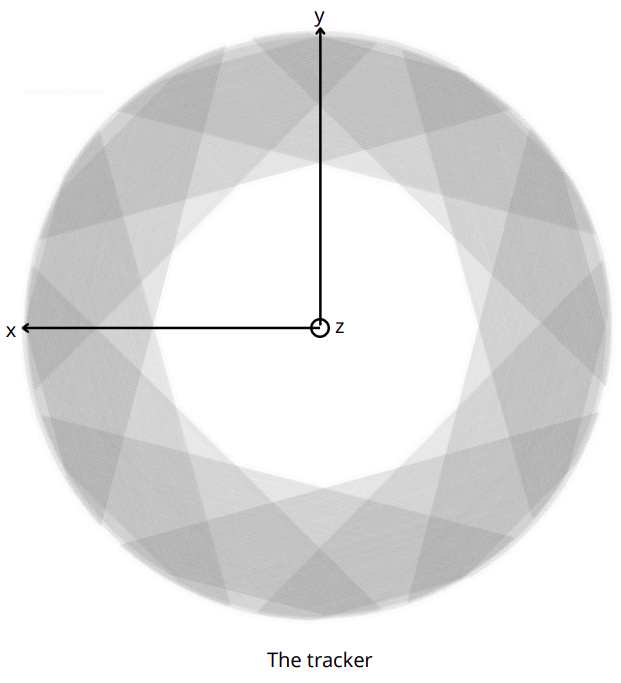
\includegraphics[width =0.6\textwidth]{figures/png/Screenshot_20240526_164527.png}
    \caption{Representation of a tracker station and definition of the coordinate used for the analysis.}
    \label{fig:coordinate}
\end{figure}
\subsection{Event selection}\label{eventselection}
Events in which a cosmic muon strikes only the first station were chosen. 

Each straw can be parametrized as a straight line
\begin{equation}\label{equaretta}
    (D_{x,i}t+M_{x,i},D_{y,i}t+M_{y,i},z_i)
\end{equation}
where $D_{x,i}$, $D_{y,i}$ are the straws' directions on $x$, $y$, while $M_{x,i}$, $M_{y,i}$ are the straws' midpoints on $x$, $y$. $z_i$ is the $z$ coordinate of the straw.
%One dimension is correlated with the other two, so we have just two informationful dimensions.
In this parametrization, the straws are all parallel on the $yz$ plane.
Since two parallel straight lines (straws) define a three-dimensional plane of possible tracks, 
at least another pair of straws, uncorrelated with the initial two, is required to reconstruct a 
single straight line. The intersection of two planes forms a straight line. Therefore, at least four straws with different $z$ coordinates are necessary, 
so a number of hits per face greater than one was required.

Since more than one hit can occur in a single panel, another selection criteria 
was to choose events with fewer than three straw hits per panel. This was chosen to minimize the error on the position reconstruction.
\subsubsection{Panels illumination pattern}
To achieve accurate timing calibration, it is essential to have uniform illumination of the hits across each panel. 
Using only the conditions outlined in Section \ref{eventselection}, the Monte Carlo hits were plotted in the reference frame of the panel. 
The result is shown in Figure \ref{fig:illumination} for panel 0 of plane 0, which corresponds to the upper right panel in Figure 
\ref{fig:coordinate}. Similar patterns were observed for all panels in both planes, as shown in Appendix \ref{appendix2}. The illumination is 
spotty and non-uniform. The reason of this strange illumination is due to the fact that the overlap areas of the panels are all on the extreme part of the panel.
Additionally, there are almost no hits in the central region, which could lead to non-linearities. 
Specifically, if particles pass near the end of the straw, the signals are wider, and wider signals have greater charge and 
height compared to others. Consequently, the leading edge would be very sharp, potentially causing timing systematics.
\begin{figure}[!h]
    \centering
    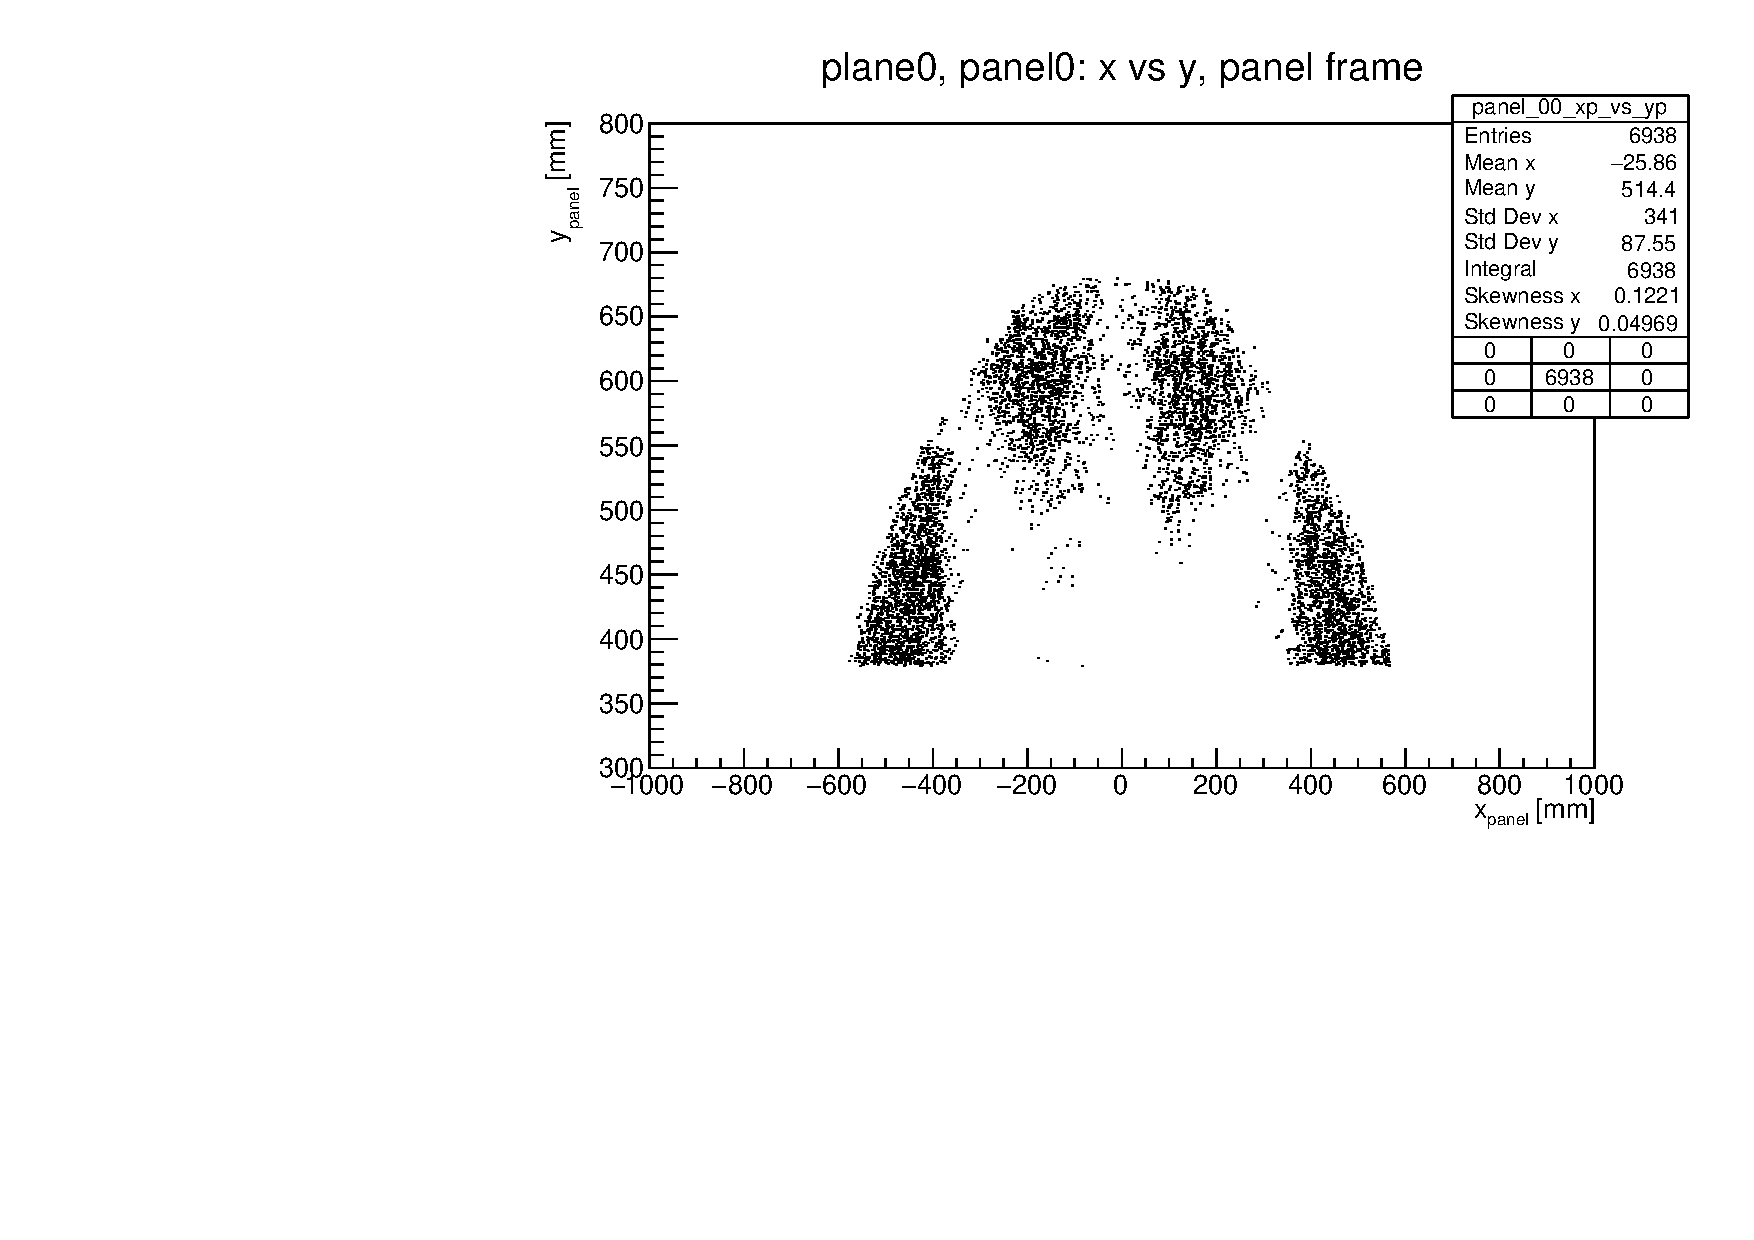
\includegraphics[width =0.8\textwidth]{figures/pdf/xp_vs_yp_panel0.pdf}
    \caption{Illumination of Monte Carlo hits on panel 0, plane 0, selecting cosmics that traverse at 
    least four panels across four distinct faces of the station, with fewer than three hits per panel.}
    \label{fig:illumination}
\end{figure}
\subsubsection{Rate}
\subsection{Reconstruction of a straight line}
Vogliamo ricostruire i segments nei cosmici partendo dal fatto che sappiamo solo se una straw e' stata colpita o meno. Sappiamo: \ref{equaretta}
\begin{itemize}
    \item mid point della straw;
    \item direzione della straw sul piano xy;
    \item posizione reciproca sulle z delle straw.
\end{itemize}
Riporto la situazione nella figura sottostante:
\begin{figure}
    \centering
    \includegraphics[width=0.8\textwidth]{Screenshot_20240423_121847.png}
    \caption{raggio cosmico che colpisce qualche straw nel panel. La direzione del cosmico non sara' mai cosi', dato che i cosmici sono distribuiti come $cos^2\theta$ e sono per lo piu' verticali.}
    \label{fig:rec}
\end{figure}
Sapendo la posizione reciproca delle straws e la loro rotazione reciproca, possiamo ricostruire il segment.
Descrivo di seguito i passaggi per ricostruire i cosmici.
Considero il midpoint di ogni straw in un panel con coordinate $(x_i,y_i,z_i)$ e la sua direzione come $(u_i,v_i,w_i)$. La direzione e' uguale a tutte le straws, quindi scrivo direttamente $(u,v,w)$ per ogni straw in un panel.
\\
Per la nostra calibrazione abbiamo scelto di utilizzare dei filtri:
\begin{itemize}
    \item dato che per ricostruire una linea retta nello spazio 3D e' necessario avere 4 punti a z diverse, abbiamo scelto di usare quegli eventi che hanno almeno una hit per face;
    \item dato che vogliamo la risoluzione su x e y essere minore di circa 4 cm sulle x e 15mm sulle y, abbiamo scelto un numero di straw colpite per panel minore uguale di 3.
\end{itemize}
Quello che posso fare con quattro panel e' ricostruite la retta che passa tra 2 punti in planes diversi, di cui ognuno e' stato costruito con una stereo tra 2 straws in 2 panels diversi. Non posso ricavare piu' di due punti, in quanto verrebbe a mancare il significato fisico (una particella che si trova in piu' di due punti in una straw contemporaneamente).
A questo punto devo ricostruire la combo hit all'interno del panel. Prendo la media dei mid points sulle x, y e z e la direzione delle straws. 
$$ (u\cdot t + x_m,v\cdot t + y_m,z_m)$$
da cui:
$$y=\frac{v}{u}(x-x_m)+y_m$$
\\
Una volta ricostruite le straw hits in combo hits, devo ricostruire le stereo hits.
Per fare questo seleziono i due panels colpiti in un plane e trovo l'intersezione tra le due straws medie trovate prima. Se ho le seguenti rette:
$$y=\frac{v_1}{u_1}(x-x_{m1})+y_{m1}$$
$$y=\frac{v_2}{u_2}(x-x_{m2})+y_{m2}$$
Il punto di incontro sara':
$$x=\frac{u_1 u_2(y_{m1}-y_{m2}+\frac{v_2}{u_2}x_{m2}-\frac{v_1}{u_1}x_{m1})}{v_2 u_1 - v_1 u_2}$$
$$y=\frac{v_2}{u_2}\left(\frac{u_1 u_2(y_{m1}-y_{m2}+\frac{v_2}{u_2}x_{m2}-\frac{v_1}{u_1}x_{m1})}{v_2 u_1 - v_1 u_2}-x_{m2}\right)+y_{m2}$$
A questo punto avro' 1 punto per plane e posso trovare la retta che passa per questi 2 punti. Chiamo i punti trovati per plane $(x_1,y_1,z_1)$ e $(x_2,y_2,z_2)$.
La retta sull'asse xy sara':
$$ m_{xy}=\frac{y_2-y_1}{x_2-x_1}$$
$$ q_{xy}=-m_{xy} \cdot x_1+y_1$$
La retta sull'asse zy sara':
$$ m_{yz}=\frac{y_2-y_1}{z_2-z_1}$$
$$ q_{yz}=-m_{yz} \cdot z_1+y_1$$
Questa linea retta interseca i 4 panels in 4 punti. Ogni panel e' definito con la propria z. Se la z viene ricavata dalla $z_i$ delle combo hits (media tra la z delle straws). Otteniamo i seguenti 4 punti:
$$ y_i=m_{yz}\cdot z_i+q_{yz}$$
$$ x_i=(m_{yz}\cdot z_i+q_{yz}-q_{xy})/m_{xy}$$
A questo punto il bias sulla posizione lungitudinale nelle straws e' dato dalla differenza tra $x_i$ e la media delle hit date dal monte carlo in un panel.



%yongi cap 3.1.5.2
%con il tracker in orizzontale , dato che le tracks sono verticali colpirebbero per panel sicuro almeno 2 straws che sono sovrappposte e quindi in totale 8, se hanno una certa angolazione anche 12






%yongi:
%As discussed in Chapter 3, the Mu2e Tracker panels need to satisfy a series of performance
%requirements for successful operations and the designed resolution. While various individual
%component and single panel tests in the past confirmed their respective effectiveness, it was of great
%interest to extend the tests to a system of multiple panels over a longer period of time under a more
%realistic setup (i.e., similar to that of the actual experiment setup), and to get better quantitative
%understandings of the detector performances. Hence, a VST was conducted.
%The overall goal of the VST was to “exercise the full tracker operation and readout chain,
%from the amplified wire signal to its storage in digitized format” [1]. The test used a whole plane of
%six panels from panel pre-production,1 which was 1/36 of the full Tracker.
%The VST contained two phases. In the first phase, the plane was laid horizontally on a
%test bench for diagnostics and horizontal position runs, as shown in Figure 5.1(a). In the figure
%the supporting systems, including gas lines, DC-to-DC converters for low voltage supplies, high
%voltage supplies, and the Raspberry Pi (marked as RPi) for panel controls, are all labeled.2 In this
%phase, the plane operations and performances were checked. The plane data output to the DAQ
%server through the optical fiber links (see Chapter 4 and Appendix B) were finalized and tested.
%Small cosmic-ray datasets werereconstruction of the track longitudinal position taken to verify the ability to synchronize data taking among the
%panels. And 55 Fe source scan studies were performed for calibrations. The second phase of the



%reconstruction of the track longitudinal position
%tracker/vstplan
%We also plan to take significant amounts of cosmic ray data in at least two configurations. First, cosmic ray data will be taken with the plane in the current horizontal
%position. This will be taken using a modified readout scheme involving the serial
%connection as described above. Software exists to take the output raw data and manually convert it into an art format that can be processed by the official Mu2e software
%packages. This first cosmic data will be used to confirm the functionality of the system - including a cross-check of the panel to panel time synchronization, and the
%overall timing measurement performance. 
%Additionally, enough statistics could allow
%for important preliminary calibrations of delta-t resolution, longitudinal propagation
%velocities, efficiencies, and channel to channel variations. The fairly uniform distribution and wide phase-space of tracks in the horizontal configuration can make these
%analyses more straightforward than in the vertical configuration. Additionally a better measure of the expected showering will allow an improved analysis of vertical data.
%Finally, it may be possible to make some measure of the difference between vertical
%and horizontal straw alignment compared to expectations from Duke measurements
%and gravitational sag
%Later, the plane will be positioned vertically and another month of cosmic data
%will be taken. At this point readout may be through the fiber and DTC for improved
%livetime. As described above we will move towards automatic processing of this
%data and have it copied and backed up to tape. This data will be most useful for
%testing the track reconstruction. There exists software for reconstructing cosmic
%tracks without a magnetic field, and it has been tested in a limited fashion with
%data from a single vertical panel (docdb-33914). The implementation for a single
%plane in either horizontal or vertical configuration is being developed.
%Finally, a more thorough calibration of the plane can be done using a systematic
%scan across each panel with an Fe55 source. This will allow further measurements of
%the response as a function of straw and position, and a determination of the variability
%between panels.